\let\negmedspace\undefined
\let\negthickspace\undefined
\documentclass[journal]{IEEEtran}
\usepackage[a5paper, margin=10mm, onecolumn]{geometry}
%\usepackage{lmodern} % Ensure lmodern is loaded for pdflatex
\usepackage{tfrupee} % Include tfrupee package

\setlength{\headheight}{1cm} % Set the height of the header box
\setlength{\headsep}{0mm}     % Set the distance between the header box and the top of the text
\usepackage{gvv-book}
\usepackage{gvv}
\usepackage{cite}
\usepackage{amsmath,amssymb,amsfonts,amsthm}
\usepackage{algorithmic}
\usepackage{graphicx}
\usepackage{textcomp}
\usepackage{xcolor}
\usepackage{txfonts}
\usepackage{listings}
\usepackage{enumitem}
\usepackage{mathtools}
\usepackage{gensymb}
\usepackage{comment}
\usepackage[breaklinks=true]{hyperref}
\usepackage{tkz-euclide} 
\usepackage{listings}
% \usepackage{gvv}                                        
\def\inputGnumericTable{}                                 
\usepackage[latin1]{inputenc}                                
\usepackage{color}                                            
\usepackage{array}                                            
\usepackage{longtable}                                       
\usepackage{calc}                                             
\usepackage{multirow}                                         
\usepackage{hhline}                                           
\usepackage{ifthen}                                           
\usepackage{lscape}
\begin{document}

\bibliographystyle{IEEEtran}
\vspace{3cm}

\title{3.2.11}
\author{EE25BTECH11065 - Yoshita.J}
% \maketitle
% \newpage
% \bigskip
{\let\newpage\relax\maketitle}

\renewcommand{\thefigure}{\theenumi}
\renewcommand{\thetable}{\theenumi}
\setlength{\intextsep}{10pt} % Space between text and floats


\numberwithin{equation}{enumi}
\numberwithin{figure}{enumi}
\renewcommand{\thetable}{\theenumi}


\textbf{Question}:\\
Draw an Right angle  triangle $\triangle ABC$ in which $\boldsymbol{BC} = 12 \text{ cm}$, $\boldsymbol{AB} = 5 \text{ cm}$, and $\angle B = 90^\circ$.
\\ \solution \\
    \begin{table}[h!]    
      \centering
      \begin{table}[h!]
    \centering
    \begin{tabular}{|c|c|}
        \hline
        Point & Coordinates \\
        \hline
	    $A$ & $\myvec{1\\-1}$ \\
	    $B$ & $\myvec{-4\\2k}$ \\
	    $C$ & $\myvec{-k\\-5}$ \\
        \hline
    \end{tabular}
    \caption{Vertices of $\triangle ABC$ before substituting $k$}
    \label{tab:triangle_k}
\end{table}

      \caption{}
    \end{table}
   \begin{align*}
      AB^2 & = 5^2 = 25, \\
      BC^2 & = 12^2 = 144.
   \end{align*}
   The squared length of AC is just the vector AC dotted with itself. In matrix form, that means multiplying the row vector (transpose) of AC with the column vector AC.
   \begin{align*}
    AC^2 &= (\vec{AC})^T (\vec{AC}) \\
         &= \myvec{12 -5} \myvec{12 \\ -5} \\
         &= (12 \times 12) + (-5 \times -5) \\
         &= 144 + 25 = 169
\end{align*}
Thus, the length of AC is:
\begin{align*}
    AC &= \sqrt{169} = 13 \text{ cm}.
\end{align*}
\newpage{}

Let's put the triangle on the coordinate plane.  
Since $\angle B$ is a right angle, we put $B$ at the origin.  \\


      $\vec{B} = \myvec{0\\0}$\\
      $\vec{A} = \myvec{0\\5}$ because $AB = 5$ cm on the $y$-axis\\
      $\vec{C} = \myvec{12\\0}$ because $BC = 12$ cm on the $x$-axis\\


    \begin{figure}[h]
       \centering
       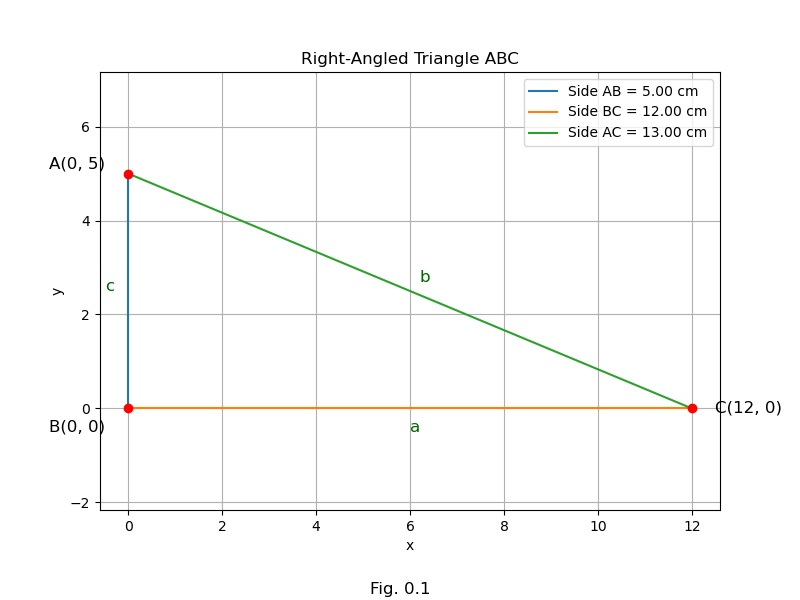
\includegraphics[width=0.9\columnwidth]{figs/fig1.png}
       \caption{}
       \label{graph}
    \end{figure}
\end{document}  

